\chapter{北京正负电子对撞机~BEPCII 和北京谱仪~BESIII}
\label{chap:bes3}
北京正负电子对撞机(BEPC)及相应的探测器北京谱仪(BES),在 ~1984 年建成。
1994 年到 1996 年加速器和探测器进行了升级,升级后的对撞机仍称为~BEPC,
而谱仪称为~BESII。
升级后,对撞机和探测器的性能均有了相当大的改进,采集了大量的~$\jpsi$、$\psip$、$\psipp$ 数据,并且对~2.0 $\sim$ 5.0\,GeV 能区进行了扫描,基于这些数据取得了许多重要的物理结果。
例如精确测量$\tau$轻子质量,对$2-5$GeV 的R值精确扫描,系统地研究粲夸克偶素的衰变等等。
从~2004 年开始,通过四年的时间~BEPC 和~BESII 进行了第二次升级改造,
2008年工程竣工,2009年开始物理取数,已经获取了世界上最大的$\tau$-粲能区$\ee$对撞数据样本。
升级后的对撞机和谱仪分别称为~BEPCII 和~BESIII\cite{BEPCBESIII_upgrade}。
现将BESIII上已经获取的实验数据信息列在表~\ref{tab:data}中,几乎所有的样本都是迄今为止世界上同一能量点统计量最大的样本。
本论文的所有研究内容都是基于BESIII探测器上获取到的对撞事例,主要是$XYZ$的数据。

本章主要介绍高能物理实验的特点以及北京正负电子对撞机和北京谱仪上的软硬件结构。

\begin{table}
\centering
\footnotesize
\caption{北京谱仪BESIII上实验数据简介。}
\begin{tabular}{lccc}
\toprule
样本名称 & 质心系能量(GeV) & 亮度或事例数 & 主要物理目标  \\
	\midrule
$\jpsi$数据    & $3.097$ & $13$亿  & 研究$\jpsi$衰变过程中产生的轻强子态性质  \\
$\psip$数据    & $3.686$ & $5$亿  & 研究粲夸克偶素之间的跃迁机制  \\
$\psipp$数据    & $3.773$ & $2.93\rm{fb}^{-1}$  & 研究粲介子的衰变性质  \\
$\tau$轻子质量扫描数据    & $3.554$ & $0.024\rm{fb}^{-1}$  &  $\tau$轻子质量的精确测量  \\
$XYZ$数据    & $3.81-4.599$ & $5\rm{fb}^{-1}$  &  奇特强子态的寻找\\
$R$值和QCD数据    & $2-3$,$3.85-4.59$ & $0.5\rm{fb}^{-1}$,$0.8\rm{fb}^{-1}$  & $R$值精确测量 \\
\bottomrule
\end{tabular}
\label{tab:data}
\end{table}


\section{粒子物理实验介绍}
粒子物理实验又称高能物理实验,主要涉及:粒子源,探测器和数据处理等方面。
早期的粒子源主要是靠来自宇宙的高能粒子射线,人们基本是“靠天吃饭”。
随着加速器技术和电子学技术的发展,人们发展了新的获取粒子源的方法, 也就是利用加速器和对撞机。
现代的粒子物理实验主要就是利用加速器将粒子加速到很高能量,然后使其对撞或打靶发生相互作用,然后用探测器探测末态的次级粒子。
对撞能量越高,能够分辨的空间距离越小,随着人们对微观结构的了解越来越深入,高能物理实验中用到的加速器能量也越来越高。
对撞实验相比于打靶实验的优势在于,两束相对运动的粒子束团对撞提高了有效作用能量,在现在的高能物理实验中,对撞实验占主导地位。

粒子探测器是记录和测量高能粒子信息的工具。高能粒子产生的事例包含不同种类的次级粒子,一般通过探测末态相对稳定的粒子 ($e,\mu,\pi,K,p,n,\gamma$) 来重建中间过程的粒子,还原整个事例的信息。
探测器根据不同粒子和物质相互作用的区别,如图~\ref{fig:tanceqi},探测末态粒子,并区分其种类。
它的具体功能是要测量反应产物的信息(位置、能量、 粒子种类等)。
这些功能通常由多个子探测器来共同完成,比如用漂移室测量带电粒子的轨迹,用电磁量能器测量中性粒子的位置和能量,
用飞行时间计数器测量粒子的飞行时间以判断粒子类型等。
通常把这种需要多个探测器协同工作的大型粒子探测装置称为谱仪。
\begin{figure}
\begin{center}
\includegraphics[width=0.5\textwidth]{chap2_general_dector}
\caption{粒子物理实验中探测器的基本工作原理示意。}
\label{fig:tanceqi}
\end{center}
\end{figure}

我们搞粒子物理实验的最终目的是要获得感兴趣的物理结果。通过合理的筛选条件处理实验获取的数据获取感兴趣的事例,就是高能实验物理分析人员要研究的事情。
经常利用粒子的四动量,对不变质量、丢失质量、动量、横动量、空间角分布、时间分布、Dalitz图等进行分析,甚至有时候还需要进行分波分析。
这些分析过程往往都需要蒙特卡洛模拟(Monte Carlo, MC)~\cite{MC}这个重要工具的帮助,以研究信号事例合理的选择条件、分析本底、得到筛选效率等。

当前粒子物理实验的三个研究前沿方向主要是:加速器物理实验的高能量、高亮度和非加速器物理的研究。
\begin{itemize}
  \item 在更高能量下寻找新粒子,探索新的物理模型~\footnote{以欧洲核子中心LHC上的几个实验为主。}。
  \item 在高亮度条件下积累大量数据,用高分辨率探测器进行精确测量,检验标准模型,寻找突破~\footnote{BESIII正是属于这一类。}。
  \item 依靠来自宇宙的高能粒子源,使用巨大体积的探测器,在低背景环境下测量低事例率的物理现象~\footnote{核电站上产生大量中微子,一些人造的非加速器对撞环境提供的粒子源均属此类。}。
\end{itemize}

\section{北京正负电子对撞机}
升级后的北京正负电子对撞机(BEPCII)是工作在$\tau$-粲能区的多束团、高亮度的正负电子对撞机,其峰值亮度比它的前身BEPC高了约两个量级。
BEPC主要由注入器,束流输运线和储存环组成。注入器是一台长202\ m的直线加速器,由电子枪产生的电子,和电子打靶产生的正电子,
被直线加速器加速后由束流输运线注入到储存环。储存环是一台环形加速器,束流在环内积累、加速、储存和对撞~\cite{BEPCII}。
BEPCII利用原有的储存环隧道,采用双环方案,使正负电子束流在两个彼此独立的储存环中积累和加速,在对撞点处对撞。
双环结构是保证亮度提高两个量级的关键选择。
BEPCII的主要性能参数列于表~\ref{tab:BEPCII}。
值得一提的是该论文完成前不久的2016年4月5日,BEPCII的亮度达到了其设计亮度$1 \times 10^{33}\rm{cm}^{-2}s^{-1}$,为工作在该能区的加速器亮度之最。
此外,北京正负电子对撞机还做到了所谓的“一机两用”,可以运行的同步辐射模式下,作为同步辐射的光源。
\begin{table}
\centering
%\footnotesize
\caption{BEPCII的主要设计参数。}
\begin{tabular}{ll}
\toprule
束流能量$E_{b}$(GeV)               &  $1.0\sim2.3$  \\
设计亮度($E_{b}$=1.89\ GeV)        &  $1 \times 10^{33}\rm{cm}^{-2}s^{-1}$ \\
高频频率(MHz)                      & 499.8 \\
对撞周期(ns)                       & 8 \\
储存环长度(m)                      & 237.53 \\
束团数目                             & 93 \\
正负电子注入速率(mA/min)           & 50 \\
\bottomrule
\end{tabular}
\label{tab:BEPCII}
\end{table}

\begin{figure}
 \centering
 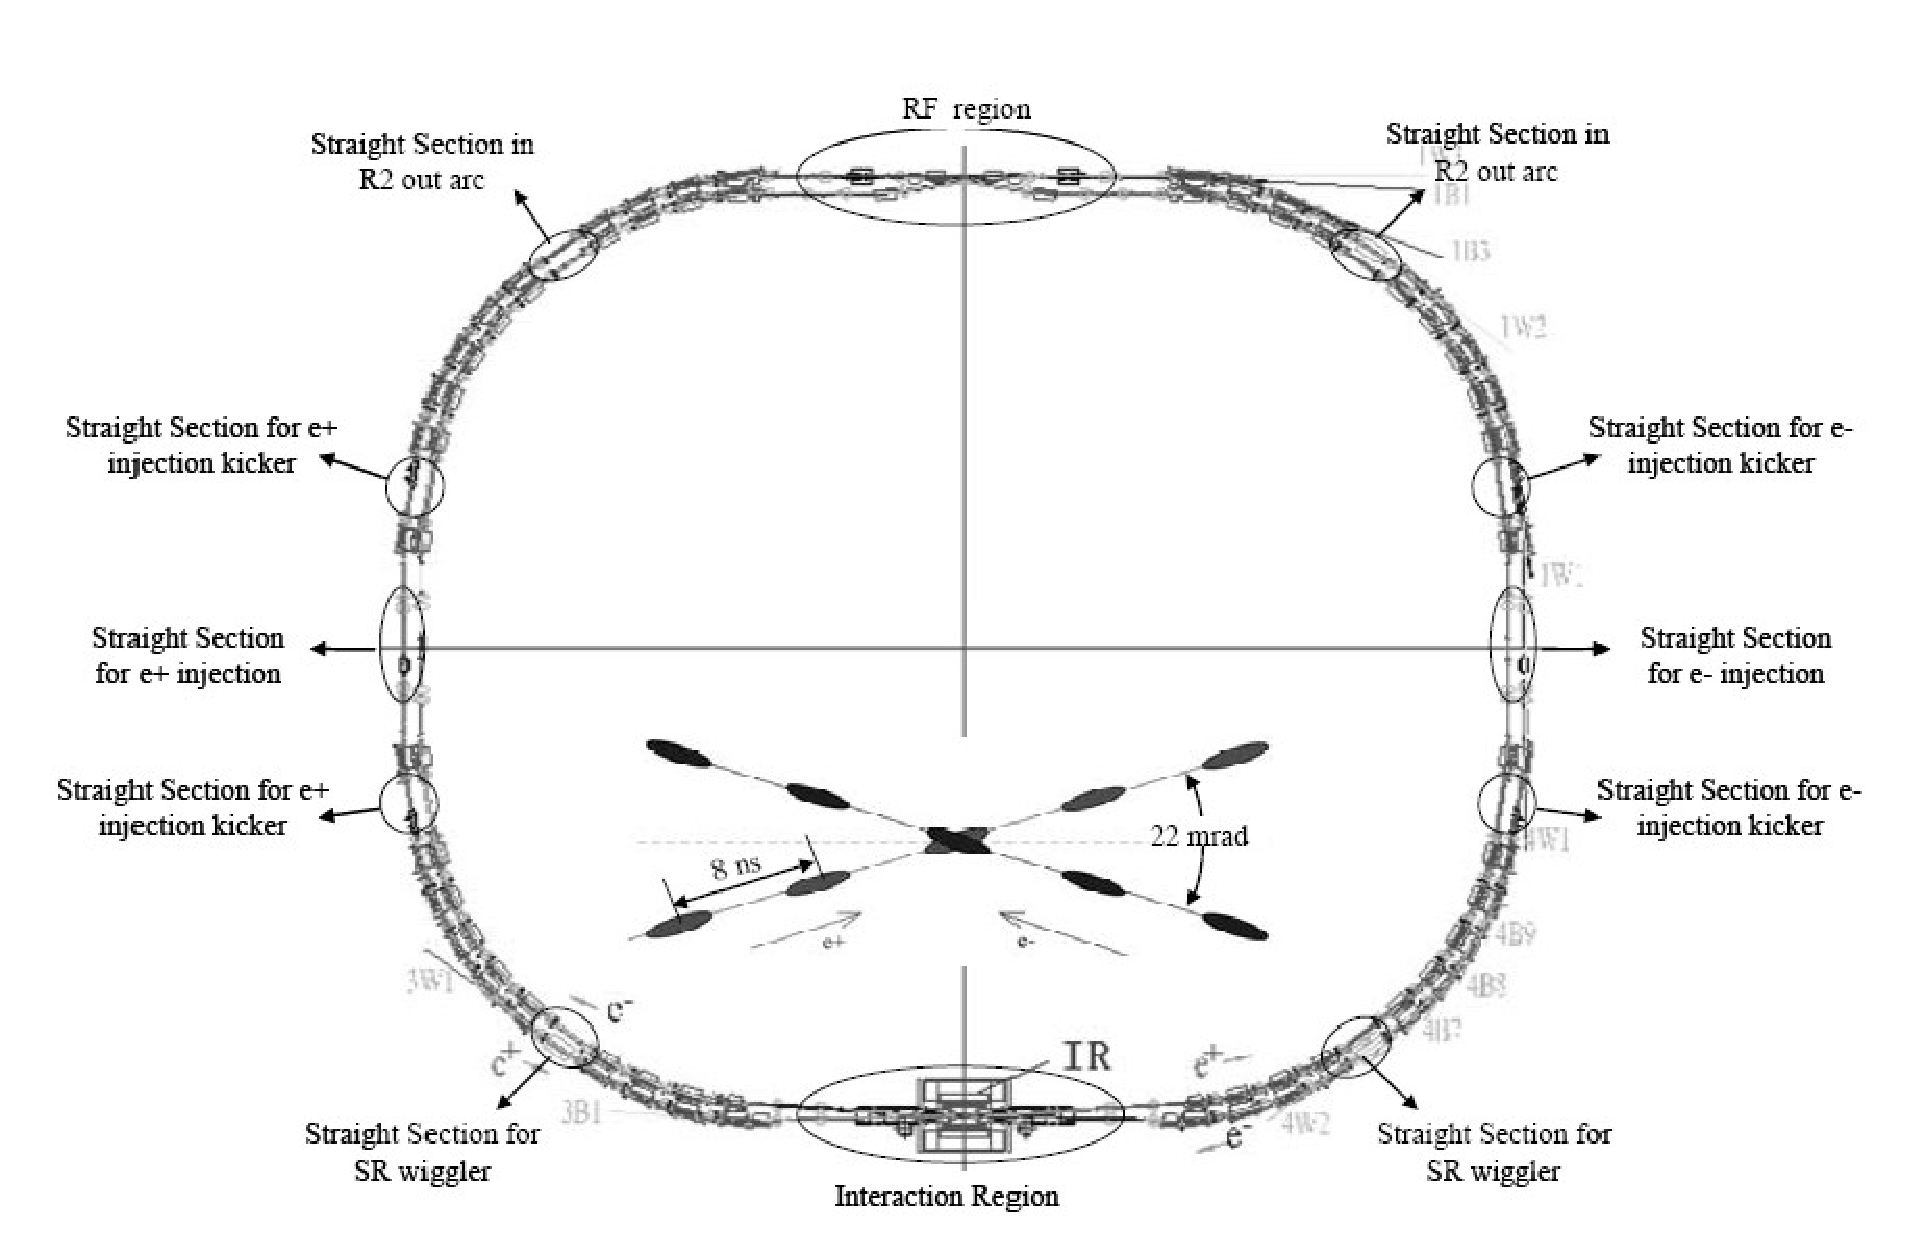
\includegraphics[width=0.8\textwidth]{chap2_BEPCII}
 \caption{BEPCII俯视图。}
 \label{fig:BEPCII}
\end{figure}

\section{北京谱仪}
北京谱仪(BESIII)是运行在BEPCII上采用现代探测技术的大型通用探测器,用于探测$e^{+}e^{-}$对撞产生的末态粒子。
BESIII工作在所谓的$\tau$-粲能区,该能区是精确检验标准模型和寻找新物理的理想场所。
BESIII的物理目标包括$\tau$-粲能区弱电相互作用的研究、强相互作用研究及新物理的寻找等~\cite{Asner:2008nq}。

BESIII将对弱电相互作用理论进行精确检验:利用$D$和$D_{s}$介子衰变精确测量CKM矩阵元,检验其幺正性;
通过精确测量$\tau$轻子质量对轻子普适性进行更高精度的检验;在$\tau^+\tau^-$近域高精度的截面测量更好地理解$\tau^+\tau^-$间的相互作用;
利用$\lambdacp\lambdacm$阈值上的优势,精确测量$\lambdacp$的强衰变和半轻衰变性质。

在强相互作用领域,由于$\tau$-粲能区强相互作用的非微扰特性,使得目前在该能区几乎所有的理论计算都有很大的不确定性。
利用$\tau$-粲能区的数据对QCD的研究主要包括:
结合高精度的LQCD的计算进行标准模型基本参数的测量,如强相互作用耦合常数$\alpha_{s}$等;测量低能强子谱, 寻找QCD预言的各种含胶子的态,如胶子球、混杂态等;
研究粲偶素的产生和衰变性质,检验和发展量子色动力学的各种计算。 

BESIII 持续高亮度的运行,使得其能够积累大量的数据,从而可以进行稀有衰变的测量,如对味道改变中性流 (FCNC)的寻找, 测量结果相对预期值的反常偏离都预示着新的机制或者新物理的贡献;还可以对非标准模型过程进行寻找,如轻子数或重子数破坏的过程。
另外,标准模型中~$D^{0}-\bar{D^{0}}$ 的混合以及~$D_{s}$/$D$ 衰变中的~CP 破坏效应都很小,而新物理的贡献可以加强这种效应。
在~BESIII 上测量中性~$D$ 介子的混合及~$CP$ 破坏,都可以用来寻找新物理或对新物理的贡献给出一个限制。


为了达到上面提到的物理目标,BESIII 探测器必须满足以下要求:
\begin{itemize}
\item 能够探测低动量的带电粒子,并精确测量其动量和方向;
\item 好的粒子鉴别能力,能够区分开各种粒子,如电子、$\mu$~子、质子、$\pi$~介子、$K$~介子等;
\item 精确测量光子,具有非常好的能量分辨、角度分辨及光子识别能力;
\item 前端电子学系统、触发系统以及数据获取系统要适应~BEPCII 多束团模式下的高事例率取数,尽量减少死时间。
\end{itemize}

基于以上要求,BESIII 探测器的总体结构如图~\ref{fig:BESIII}所示。
由内向外依次为主漂移室(Main Drift Chamber, MDC)、飞行时间计数器(Time of Flight, TOF)、CsI电磁量能器(Electro-Magnetic Calorimeter, EMC)、 超导磁体(Superconductor Magnet)和$\mu$子计数器(Muon Counter, MUC)。
表~\ref{tab:bes3p}给出了BESIII探测器的主要性能参数~\cite{BESIII}。

\begin{figure}
 \centering
 \includegraphics[angle=90,width=0.8\textwidth]{chap2_bes_view}
 \caption{BESIII探测器的结构侧视图。}
 \label{fig:BESIII}
\end{figure}


\begin{table}
\centering
\footnotesize
\caption{BESIII主要性能参数。}
\begin{tabular}{ll}
\toprule
子系统                         & 主要性能参数 \\
\midrule
\multirow{3}* {主漂移室}       & $\sigma_{xy}$=130\ $\mu$m            \\
                               & $\Delta P$/{\it{P}}=0.5\ \% @1.0\ GeV     \\
                               & $\sigma_{dE/dx}$=6-7\ \%              \\
\midrule
\multirow{2}* {飞行时间计数器} &  $\sigma_{t}$= 90\ ps 桶部  \\
                               &  $\sigma_{t}$= 110\ ps 端盖  \\
\midrule
\multirow{2}* {电磁量能器}     &  $\Delta E$/{\it{E}}=2.5\ \% @1.0\ GeV  \\
                               &  $\sigma_{\phi z}$=0.6\ cm  @1.0\ GeV  \\
\midrule
$\mu$ 子计数器                 &   9\ 层   \\
磁场强度                       &   0.9 $\sim$ 1.0\ T \\
\bottomrule
\end{tabular}
\label{tab:bes3p}
\end{table}

\section{小结}
本章简要介绍了BEPCII和BESIII的结构、BESIII 各个子系统的结构性能和指标等。
